\section{Cloud Storage}


\subsection{Storage models}
    In cloud computing a massive amount of data needs to be handled. If years ago the most important service was the performance of cloud, nowadays it' reliability: data has to be stored and providers have to be able to make sure to not lose them.
    In order to provide reliability, different copies of the same data will be stored. The disadvantage is that maintaining consistency among multiple copies of data will require more software complexity.
    
    We define \textbf{storage model} the layout of a data structure in a physical storage.
    
    We define \textbf{data model} the set of logical aspects related to how to store data in a given space.
    
    Storage models must guarantee two features:
    \begin{itemize}
        \item Storage models must be \textbf{read/write coherent}: the result of a read operation of memory should be the same as the most recent write operation; in other words every operation of read operation needs to ensure that the previous write operation has been already completed.
        \item Storage models must respect the \textbf{before-or-after atomicity}: the result of an operation, from the point of view of the invoker, must be the same as if the actions occurred either completely before or completely after.
    \end{itemize}

    
\subsection{Block storage}
    Data are managed by means of blocks within sectors and tracks (this is very useful mostly for databases by DBMS).
    
    OpenStack Cinder is a Block Storage service for OpenStack. It's designed to present storage resources to end users, in particular it allows to interact with different row and not formatted hardware. 
    
    \begin{figure}[h!]
        \centering
        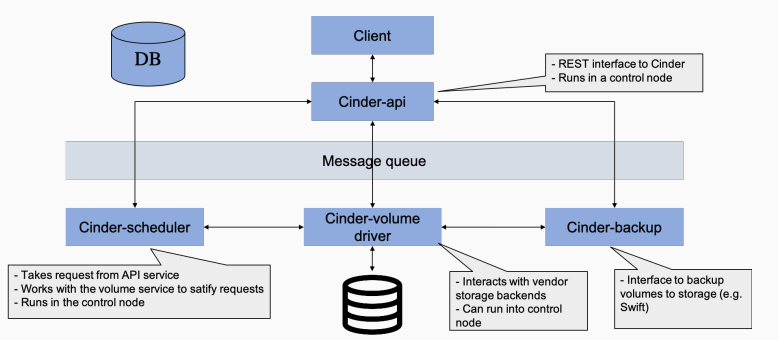
\includegraphics[scale=0.5]{images/Cinder architecture.png}
    \end{figure}
    
    The Cinder architecture is composed by:
    \begin{itemize}
        \item a volume driver that interacts with the vendor
        \item a scheduler that takes request from the API interface (like modifying a volume and snapshots).
        \item a backup that is an interface for backupping volumes.
    \end{itemize}


% -------------------


\subsection{Distributed file systems}

At first let's introduce some term.
\begin{itemize}
    \item \textbf{A file} is a linear array of cells stored on a persistent storage device, is viewed by an application as a collection of logical record and is stored on a physical device as a set of physical records of size dictated by the physical media.
    \item \textbf{A file pointer} is a cell used as a starting point for a read or write operation
\end{itemize}
A file could be organised as:
\begin{itemize}
    \item \textbf{Logical}: reflects the data model, the view of the data from the prospective of the application
    \item \textbf{Physical}: reflects the storage model and describes the manner the file is stored on a given storage media
\end{itemize}

So a \textbf{file system} is a collection of directories, each directory provides information about a set of files it could be \textit{traditional} (like the Unix File System) or \textit{distributed} (like the Network File System ...).

\subsubsection{Unix File System}
The Unix File System is based in three main points:
\begin{itemize}
    \item \textit{Layered} design provide flexibility
    \begin{itemize}
        \item Layered design allows UFS to separate the concerns for the physical structure from the logical one
        \item \textit{inode} layer allows UFS to treat uniformly local and remote file access
    \end{itemize}
    \item \textit{Hierarchical} design supports scalability reflected by the file naming convention (like nested directory)
    \item \textit{Metadata} supports a systematic design philosophy of the file system and device-independence
    \begin{itemize}
        \item Metadata includes information like file owner, access rights, creation time ecc. (these information are very useful for managing files)
        \item inodes contains information about individual files and directories
    \end{itemize}   
\end{itemize}   

Let's add some knowledge in the USF layering:
The lower layers are for the physical organization
\begin{itemize}
    \item Block layer: to locate individual blocks on the physical device
    \item File layer: reflects organization of blocks into files
    \item Inode layer; provides metadata for the objects
\end{itemize}
The upper layers are for logical organization and the File name layer mediates between machine and user oriented view of the FS.
\begin{figure}[h!]
    \centering
    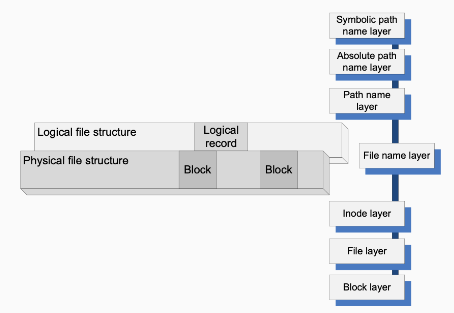
\includegraphics[scale=0.35]{images/UFSlayering.png}
    \caption{UFS layering}
    \label{fig:usfl}
\end{figure}

\subsubsection{Network File System}
The design objectives are:
\begin{itemize}
    \item Provide the same semantics as a local Unix File System (UFS) to esnure compatibility
    \item Facilitate easy integration into existing UFS
    \item Support clients running on different operating system 
    \item Accept a modest performance degradation due to remote access
\end{itemize}
NFS is based on the Client-Server paradigm so Client runs on the local host while the server is at the site of the remote file system, they interact by means of Remote Procedure Calls (RPC). In the NFS a remote file is uniquely identified by a file handle instead of a file descriptor.

\begin{figure}[h!]
    \centering
    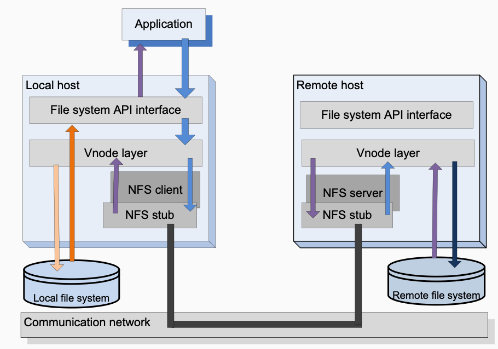
\includegraphics[scale=0.35]{images/NFS.png}
\end{figure}

The vnode layer (corresponding of inode) implements file operation in a uniform manner, regardless of whether the file is local or remote, the steps for a client-server interacrion are simple: NFS client packages the relevant information about the target, NFS server passes it to the vnode layer on the remote host and finally remote vnode layer directs it to the remote file system.

\subsubsection{Design for distributed file system}
In general  common policy is once file is closed, server will have the newest version on persistent storage. The policy to write a block are: \textit{write-backs}: a block is first written to cache and writing on the disk is delayed for a time in the order of tens of seconds, this speeds-up writing but could be cause of lost of data if the system fail. In \textit{write-through}: block is written to the disk as soon as it is available on the cache. Another point is the concurrency.

\subsubsection{Google File System}
The Google File System was developed in the late 90s, the design consideration are
\begin{itemize}
    \item Scalability and reliability are critical
    \item Vast majority of files range in size from a few GB to hundreds of TB
    \item Most common operation is to append an existing file 
    \item Sequential read operation are the norm
    \item Segment a file in large chunks 
    \item Build cluster around high-bandwidth, separate control from data flow, use TCP connections 
    \item Eliminate caching at the client site, is only on server side
    \item Have a master that control the entire cluster, we have to communicate with it to "enter" the cluster
\end{itemize}
We say that GFS uses chunks, they are fixed-size segments of 64 MB, this beacuse we have to store large file and this optimize this (and reduces the amount of metadata) and doing this multiple likelihood operations will be directed to the same chunk. Chunks are stored on Linux File System and are replicated on multiple sites. At the time of file creation each chunk is assigned a unique chunk handle.

\begin{figure}[h!]
    \centering
    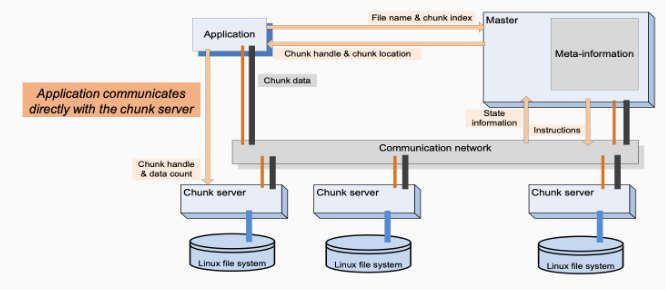
\includegraphics[scale=0.35]{images/GFS arch.png}
\end{figure}

The master maintains state information about all system components.

Let's see how a write request is performed:
\begin{itemize}
    \item Client contacts the master which assigns a lease to one of the chunk servers 
    \item Master replies with the ID of the primary and secondary chunk servers holding replicas of the chunk
    \item Client sends data to all chunk servers holding replicas
    \item Client send write request to primary chunk server once it got acks from all chunk server holding replicas
    \item Primary chunk server sends write to all secondaries
    \item Each secondary applies mutations in the order of the sequence number and sends ack back to primary
    \item After receiving ack from all secondaries, primary acks client
\end{itemize}

\subsection{Locks and consensus}
Operating systems use lock managers to organise and serialise access to resources, locks enable controlled access to shared storage and ensure atomicity of read and write operations. To elect a leader or a reliable master to take decisions, consensus must be sometimes reached.
The locks are discriminated for the \textbf{effect}
\begin{itemize}
    \item \textbf{Advisory locks}: based on the assumption that all processes play by the rules, all file can have the access of the file
    \item \textbf{Mandatory locks}: block access to the locked objects to all processes that do not hold the locks
\end{itemize}
or for \textbf{Time}
\begin{itemize}
    \item \textbf{Fine-grained locks}: locks that can be held for only a very short time 
    \item \textbf{Coarse-grained locks}: locks held for a longer time
\end{itemize}

\subsubsection{Chubby}
Chubby is a lock service developed by Google, is developed for a large number of machines connected by high-speed network, chubby provides an interface much like a distributed file system, it's an \textbf{advisory lock} and uses PAXOS\footnote{It's a family of protocols for solving consensus problems in a network} to ensure liveness.

The design of chubby it's not complicated, it consist of two main component that communicate via RPC (a replica server and a library). Chubby cell consists of a small set of servers (tipically 5, this for not having a tie when reaching the consens) known as replicas, they use PAXOS to elect a master and replicate logs, read and write requests are satisfied by the master alone.
\begin{figure}[h!]
    \centering
    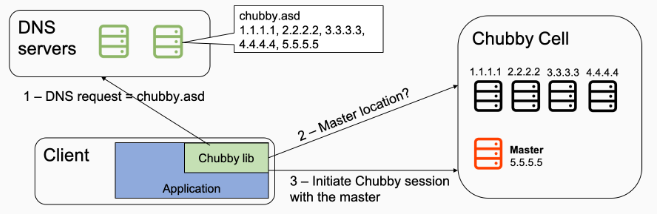
\includegraphics[scale=0.35]{images/chubbydesign.png}
\end{figure}

Chubby exports a file system interface simpler than Unix, tree of files and directories with name components separated by /, each directory contains a list of child files and directories 

\begin{table}[h!]
    \centering
    \begin{tabular}{c c c}
          ls / & asd / & dunno/nothingJS\\
          is a prefix common & name of the & is the named chubby cell\\
          to all chubbys (lock service) & chubby cell 
    \end{tabular}
\end{table}

A node is a file or directory, they can be either permanent or ephemeral, they have metadata and handlers.

So chubby is a distributed lock service for coarse-grained synchronization of distributed systems.

\subsection{Distributed databases}
Google big table (GBT) is a distributed storage system for managing structured data, is designed to scale to a very large size, is not a relational database, it more a key/value mapping, bigtable is a flexible, high performance solution.

\begin{figure}[h!]
    \centering
    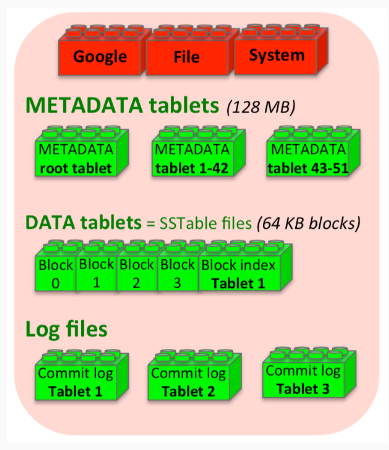
\includegraphics[scale=0.35]{images/GBTstruct.png}
\end{figure}    

It is made by Google file system, Metadata tablets, Data tablets and log files.

%SE HAI DI MEGLIO TE DI STA PARTE MI FARESTI UN FAVORE AHHAHA [pag 49 50 51]

A thing we have to know is that if Chubby is unavailable then Bigtable is Unavailable.

The major components of GBT are:
\begin{itemize}
    \item One \textbf{Master} server: it assigning tablets to tablet servers, detecting the addition and expiraiton of tablet server, balancing tablet server load, Garbage collecting of files in GFS and Handling schema changes.
    \item Many \textbf{Tablet} servers: each manages a set of tablets, handles read and write request to the tablets and splits tablets that have grown too large
    \item \textbf{Client}: Do not rely on the master for tablet location and information and communicates directly with tablet servers for reads and writes
\end{itemize}
Each tablet is assigned to one tablet server at time, when a tablet is unassigned, master assigns the tablet to an available tablet server by sending a tablet load request. When a tablet server starts it creates and acquires an exclusive lock on a uniquely-named file in a specific Chubby directory. A tablet server stops serving its tablets if it loses its exclusive Chubby lock. Master is responsable for detecting when a tablet server is no longer serving its tablets. To ensure that a Bigtable cluster is not vulnerable to networking issues if the master's Chubby session expires it will kills itself.
%QUESTA PARTE LA FINISCO DOMANI